\documentclass[bimj,fleqn]{w-art}
\usepackage{times}
\usepackage{w-thm}
\usepackage[authoryear]{natbib}
\setlength{\bibsep}{2pt}
\setlength{\bibhang}{2em}
\newcommand{\J}{J\"{o}reskog}
\newcommand{\So}{S\"{o}rbom}
\newcommand{\bcx}{{\bf X}}
\newcommand{\bcy}{{\bf Y}}
\newcommand{\bcz}{{\bf Z}}
\newcommand{\bcu}{{\bf U}}
\newcommand{\bcv}{{\bf V}}
\newcommand{\bcw}{{\bf W}}
\newcommand{\bci}{{\bf I}}
\newcommand{\bch}{{\bf H}}
\newcommand{\bcb}{{\bf B}}
\newcommand{\bcr}{{\bf R}}
\newcommand{\bcm}{{\bf M}}
\newcommand{\bcf}{{\bf F}}
\newcommand{\bcg}{{\bf G}}
\newcommand{\bcs}{{\bf S}}
\newcommand{\bca}{{\bf A}}
\newcommand{\bcd}{{\bf D}}
\newcommand{\bcc}{{\bf C}}
\newcommand{\bce}{{\bf E}}
\newcommand{\ba}{{\bf a}}
\newcommand{\bb}{{\bf b}}
\newcommand{\bc}{{\bf c}}
\newcommand{\bd}{{\bf d}}
\newcommand{\bx}{{\bf x}}
\newcommand{\by}{{\bf y}}
\newcommand{\bz}{{\bf z}}
\newcommand{\bu}{{\bf u}}
\newcommand{\bv}{{\bf v}}
\newcommand{\bh}{{\bf h}}
\newcommand{\bl}{{\bf l}}
\newcommand{\be}{{\bf e}}
\newcommand{\br}{{\bf r}}
\newcommand{\bw}{{\bf w}}
\newcommand{\de}{\stackrel{D}{=}}
\newcommand{\bt}{\bigtriangleup}
\newcommand{\bfequiv}{\mbox{\boldmath $\equiv$}}
\newcommand{\bmu}{\mbox{\boldmath $\mu$}}
\newcommand{\bnu}{\mbox{\boldmath $\nu$}}
\newcommand{\bxi}{\mbox{\boldmath $\xi$}}
\newcommand{\btau}{\mbox{\boldmath $\tau$}}
\newcommand{\bgamma}{\mbox{\boldmath $\Gamma$}}
\newcommand{\bphi}{\mbox{\boldmath $\Phi$}}
\newcommand{\bfphi}{\mbox{\boldmath $\varphi$}}
\newcommand{\bfeta}{\mbox{\boldmath $\eta$}}
\newcommand{\bpi}{\mbox{\boldmath $\Pi$}}
\newcommand{\bequiv}{\mbox{\boldmath $\equiv$}}
\newcommand{\bvarepsilon}{\mbox{\boldmath $\varepsilon$}}
\newcommand{\btriangle}{\mbox{\boldmath $\triangle$}}
\newcommand{\bdelta}{\mbox{\boldmath $\Delta$}}
\newcommand{\beps}{\mbox{\boldmath $\epsilon$}}
\newcommand{\btheta}{\mbox{\boldmath $\theta$}}
\newcommand{\balpha}{\mbox{\boldmath $\alpha$}}
\newcommand{\bsphi}{\mbox{\boldmath $\varphi$}}
\newcommand{\bsig}{\mbox{\boldmath $\sigma$}}
\newcommand{\bfpsi}{\mbox{\boldmath $\psi$}}
\newcommand{\bfdelta}{\mbox{\boldmath $\delta$}}
\newcommand{\bsigma}{{\bf \Sigma}}
\newcommand{\bzero}{{\bf 0}}
\newcommand{\bpsi}{\mbox{\boldmath $\Psi$}}
\newcommand{\bep}{\mbox{\boldmath $\epsilon$}}
\newcommand{\bomega}{\mbox{\boldmath $\Omega$}}
\newcommand{\bfomega}{\mbox{\boldmath $\omega$}}
\newcommand{\blambda}{\mbox{\boldmath $\Lambda$}}
\newcommand{\bflambda}{\mbox{\boldmath $\lambda$}}
\newcommand{\bfsigma}{\mbox{\boldmath $\sigma$}}
\newcommand{\bfpi}{{\mbox{\boldmath $\pi$}}}
\newcommand{\bupsilon}{\mbox{\boldmath $\upsilon$}}
\newcommand{\obs}{{\rm obs}}
\newcommand{\mis}{{\rm mis}}
\theoremstyle{plain}
\newtheorem{criterion}{Criterion}
\theoremstyle{definition}
\newtheorem{condition}[theorem]{Condition}
\usepackage[]{graphicx}
\chardef\bslash=`\\ % p. 424, TeXbook
\newcommand{\ntt}{\normalfont\ttfamily}
\newcommand{\cn}[1]{{\protect\ntt\bslash#1}}
\newcommand{\pkg}[1]{{\protect\ntt#1}}
\let\fn\pkg
\let\env\pkg
\let\opt\pkg
\hfuzz1pc % Don't bother to report overfull boxes if overage is < 1pc
\newcommand{\envert}[1]{\left\lvert#1\right\rvert}
\let\abs=\envert


% own packages

% kableExtra
\usepackage{booktabs}
\usepackage{longtable}
\usepackage{array}
\usepackage{multirow}
\usepackage{wrapfig}
\usepackage{float}
\usepackage{colortbl}
\usepackage{pdflscape}
\usepackage{tabu}
\usepackage{threeparttable}
\usepackage{threeparttablex}
\usepackage[normalem]{ulem}
\usepackage{makecell}
\usepackage{xcolor}

\begin{document}

%\DOIsuffix{bimj.DOIsuffix}
\DOIsuffix{bimj.200100000}
\Volume{52}
\Issue{61}
\Year{2020}
\pagespan{1}{}
\keywords{Model-Based Optimization; Design of Experiments;\\ %FIXME: name 5 %Up to five keywords are allowed and should be given in alphabetical order. Please capitalize the key
\noindent \hspace*{-4pc}\\
\hspace*{-4pc} {\small\it words)}\\[1pc]
\noindent\hspace*{-4.2pc} Supporting Information for this article is available from the author or on the WWW under\break \hspace*{-4pc} \underline{http://dx.doi.org/10.1022/bimj.XXXXXXX} (please delete if not
applicable)
}  %%% semicolon and fullpoint added here for keyword style

\title[Model-based Optimization of Adaptive Seamless Designs]{Optimizing the power of adaptive seamless designs using Bayesian Optimization} %(please use sentence case, e.g. Score tests for exploring complex models)
%% Information for the first author.
\author[Jakob Richter {\it{et al.}}]{Jakob Richter\footnote{Corresponding author: {\sf{e-mail: richter@statistik.tu-dortmund.de}}}\inst{,1}} 
\address[\inst{1}]{Fakultät Statistik, Technische Universität Dortmund, 44221 Dortmund}
%%%%    Information for the second author
\author[dd]{Tim Friede\inst{2}}
\address[\inst{2}]{Institut für Medizinische Statistik, Universitätsmedizin Göttingen, 37073 Göttingen}
%%%%    Information for the third author
\author[]{Jörg Rahnenführer\inst{1}} %please provide full author names. Middle names should be indicated by initials only, i.e. Henry J. James
%%%%    \dedicatory{This is a dedicatory.}
\Receiveddate{zzz} \Reviseddate{zzz} \Accepteddate{zzz} 

% max 250 words
\begin{abstract}
Planning the patient group sizes and test methods for clinical trials in such a way that the test power is as high as possible for given effect sizes under the null hypothesis and for a fixed number of treatments is a crucial task.
From a wide set of possible setups we want to chose the most promising plan in short time to drive fast decisions.
While it is possible to simulate the power for all various setups, the space of possible setups soon becomes too big.
Either you need big computational resources or you have to wait for an exhaustive exploration of the possible setups.
In this paper we show that you can successfully apply Model-based Optimization to find a clinical trial set-up that yields a high power from a wide set of possible set-ups.
We demonstrate the effectiveness of our approach by optimizing the power of adaptive seamless designs for different sets of treatment effect sizes and compare the result to an exhaustive search to show that our optimization approach finds a promising setup in a fraction of the time.
\end{abstract}



%% maketitle must follow the abstract.
\maketitle                   % Produces the title.

%% If there is not enough space inside the running head
%% for all authors including the title you may provide
%% the leftmark in one of the following three forms:

%% \renewcommand{\leftmark}
%% {First Author: A Short Title}

%% \renewcommand{\leftmark}
%% {First Author and Second Author: A Short Title}

%% \renewcommand{\leftmark}
%% {First Author et al.: A Short Title}

%% \tableofcontents  % Produces the table of contents.


\section{Introduction}

Clinical research and in particular drug development is typically structured into phases, e.g. phases I to IV in drug development; similar approaches for e.g. complex interventions (MRC framework). 
The development phases include elements of learning and confirmation. 
For instance, \citet{sheiner_learning_1997} described the drug development process as two learning and confirming cycles. 
First learning / confirming cycle (Phase I-IIa): Learning about tolerated dose (Phase I). 
Then confirming of efficacy of selected dose in selected group of patients (Phase IIa). 
Second learning / confirming cycle (Phase IIb-III): Learning about optimal use in representative patients (Phase IIb); Then confirming of acceptable benefit / risk ratio (Phase III). 
Traditionally, separate studies for learning and confirming.  

Changing landscape in clinical research: Dissolving boundaries between development phases; Master protocols: Broader developments focusing not only on one single treatment or one single indication / disease; Adaptive designs: Study designs become more flexible; More principled approach to decision making using statistical modeling and integrated analyses across studies

More complex designs and analyses of clinical trials. 
Examples: adaptive design; evidence synthesis.

With increasing complexity of both designs and analyses of clinical trials the planning of such studies often relies on computer simulations, since no closed form solutions even for usually fairly straightforward tasks as sample size calculations are available. 
Frameworks and guidance have been developed over the past years on how to planning, execution and interpretation of such simulation studies. 
Method comparison studies (references), references on simulation studies, in particular Clinical Scenario Evaluation (CSE).

Depending on the setting and the purpose of the simulation study suitable metrics are chosen to compare alternative design or analysis strategies. 
While method comparison studies aim to make statements when one approach might dominate others in terms of the chosen metrics, in designing an individual study or series of studies the objective is to identify a design that is optimal in terms of the metrics chosen in a certain scenario or, more importantly, across a set of scenarios. 
Here we propose to use a formal approach to optimization. 
The set of possible scenarios can be described as a multi dimensional search space, including real-valued and categorical parameters.
This vast space of possible setups makes the optimization computationally demanding.
We demonstrate here, that the use of the so-called Model-based Optimization (MBO) approach~\citep{jones_taxonomy_2001} can be applied successfully to maximize the statistical power of a clinical trial design for given effect sizes and number of treatments.

The remainder of the manuscript is structured as follows:


%\subsection{Related work}
%subsub Clinical 
% TODO: Tim

Model-based optimization, or often used interchangeably Bayesian optimization has been successfully applied to optimize expensive black-boxes in many scenarios.
Popular applications include hyper-parameter tuning of machine learning methods~\citep{snoek_practical_2012}, general algorithm configuration~\citep{hutter_sequential_2011}, and many more.
Various implementations of Model-based optimization methods are used widely, such as SMAC~\citep{hutter_sequential_2011}, Spearmint~\citep{snoek_practical_2012} and BoTorch~\citep{balandat_botorch_2020}.
For this work we use the implementation in the R-package mlrMBO~\citep{bischl_mlrmbo_2017}.
This implementations has been successfully applied to optimize hyper-parameters of machine learning methods on various tasks~\citep{bischl_mlrmbo_2017, wozniak_candle_2018}, and in the biomedical context it has been applied to optimize model-weights~\citep{richter_modelbased_2019,browaeys_nichenet_2020}.

\section{Motivating Example}
% TODO: Jakob 
% phase 1 idea something fast
% phase 2
% Describe the study we look at. / The Data
COPD trial
% Friede et al (2020) Biom J, Section 5.1 Clinical trial in COPD with treatment selection;
\cite{friede_adaptive_2020}

% What about these three papers?
\cite{barnes_integrating_2010}
\cite{donohue_oncedaily_2010}
\cite{cuffe_when_2014}

% Do we really take in this Assurance?
Assurance: \cite{stallard_optimal_2009}

\section{Adaptive Seamless Designs}
% TODO: Jakob copy contents from paper
% TODO: Tim
Intro 3- 4 Sätze

\subsection{Two-stage design with treatment selection}
Multi-arm trial; two-stages; treatment selection in interim analysis; final analysis based on combination test approach with closed test principle

% first stage = interrim analysis
% second stage = final analysys
% stick to first second stage througout text but mention interrim here?

\subsection{Selection rules}
\paragraph{Epsilion Rule}

\paragraph{Threshold Rule}

\subsection{Clinical scenario evaluation for ASD}
Friede et al (2010) DIJ, Figure 2

\subsection{Simulating ASD}
R package asd by Nick Parsons
Test statistics are simulated, not individual participant data

\section{Model-based Optimization}

Sequential \textbf{Model-based Optimization (MBO)}~\citep{jones_taxonomy_2001} (also known as Bayesian optimization) is a state-of-the-art~\citep{shahriari_taking_2016} technique for expensive black-box optimization problems.
In comparison to other black-box optimization methods, like Genetic Algorithms or Simulated Annealing, MBO is especially suitable when evaluating a configuration (e.g.\ running a simulation with certain parameters, here denoted by $\theta$) is very time consuming, and it becomes infeasible to evaluate the black-box for thousands of configurations.
MBO solves the optimization problem within a bounded search space $\Theta$:
\[
\theta^\ast := \operatorname{arg\,max}_{\theta \in \Theta} f(\theta),
\]
where $f(\theta)$ denotes the evaluation of the black-box with the input configuration $\theta$.
To reduce the number of evaluations on $f$ the key idea of MBO is to only evaluate values of $\theta$ that are estimated to lead to a small value of $f(\theta)$.
The estimate is generated by a so called \emph{surrogate model}.
Typically, this is a regression model that predicts the outcome of $f$ based on previous evaluations of $f$.
First, an initial design of already evaluated configurations is needed.
Then, iteratively, the MBO algorithm fits the surrogate on the previous evaluations, proposes a new configuration $\theta$ and evaluates it on $f$.
The steps are repeated until a budget is exhausted.

The proposal of a new configuration $\theta$ is obtained by maximizing a so called acquisition function.
The acquisition function guides the search to promising new regions in the search space $\Theta$ by facilitating the mean prediction $\hat{\mu}(\theta)$ as well as the uncertainty prediction $\hat{s}^2(\theta)$ of the surrogate.
It balances between exploration of not yet evaluated regions in $\Theta$ and exploitation.
The acquisition function achieves exploration by giving a high value to areas where the surrogate predicts a high uncertainty.
Exploitation is achieved by giving high values to values of $\theta$ where the surrogate predicts a high outcome of $f$.
For deterministic functions the expected improvement~\citep{jones_efficient_1998} is arguably the most popular acquisition function.

\paragraph{Acquisition function for noisy outcomes}
Since this work focuses on optimization of a stochastic simulation, we assume that our non-deterministic optimization problem can be formulated as follows:
\begin{equation}
\theta^\ast := \operatorname{arg\,max}_{\theta \in \Theta} f(\theta) + \varepsilon \, \text{,with}  \varepsilon \sim N(0, \sigma^2_{n}) \text{iid.}
\end{equation}
In this setting the expected improvement is not feasible as shown in \citet{huang_global_2006}.
They propose to use the augmented expected improvement instead.
Therefore, in a first step, we calculate the \emph{effective best solution}:
\begin{equation}
  \theta^{\ast\ast} := \operatorname{arg\,max}\limits_{\theta \in \mathcal{D}} \hat{\mu}(\theta) - c \cdot \hat{s}(\theta),
\end{equation}
with $c$ as a tuning parameter that is usually set to 1 and $\mathcal{D}$ as the design that contains all previously evaluated values of $\theta$.
The effective best point is the pessimistic estimate of the best observed outcome so far.
In the final step, we calculate the augmented expected improvement~\citep{huang_global_2006} as follows:
\begin{multline}
  \label{eq:aei}
  \operatorname{AEI}(\theta) = \left( \hat{\mu}(\theta) - \hat{\mu}(\theta^{\ast\ast}) \right) \cdot  \Phi \biggl( \frac{\hat{\mu}(\theta) - \hat{\mu}(\theta^{\ast\ast})}{\hat{s}(\theta)} \biggr) \\
   + \hat{s}(\theta) \cdot \phi \biggl( \frac{\hat{\mu}(\theta) - \hat{\mu}(\theta^{\ast\ast})}{\hat{s}(\theta)} \biggr) \cdot \biggl(1 - \underbrace{\frac{\sigma_{n}}{\sqrt{\sigma_{n}^2 + \hat{s}^2(\theta)}}}_{\text{correction}}\biggr),
\end{multline}
with $\Phi$ and $\phi$ as the distribution and density function of the standard normal distribution, and
with $\sigma_{n}^2$ denoting the random error (nugget effect) in the Kriging model.
The formula is derived under the assumption, that at each point $\theta \in \Theta$ the posterior of the function outcome follows a normal distribution.
This assumption is also reflected by using a Gaussian process regression as a surrogate.
However, the intuition in this formula is that the first summand favors exploitation while the second summand favors exploration.
The correction term is necessary to avoid exploration in areas where the model uncertainty ($\hat{s}^2(\theta)$) equals the random error ($\sigma_{n}^2$), because in this case further evaluations will not decrease the model uncertainty.

\paragraph{Choosing the best point from noisy outcomes}
If we chose the configuration ($\theta$) from all previously evaluated configurations that led to the best outcome of $f$ as the optimization result, we would be overly optimistic.
It is likely that a single best outcome can be attributed to the random error ($\sigma_{n}^2$).
Instead we are interested in the optimum of the true posterior mean.
Therefore, we employ the surrogates estimate of the posterior mean for each evaluated configuration to cancel out the noise.
The configuration for which the surrogate estimates the best outcome is then returned as the optimization result $\hat{\theta}^\ast$:
\begin{equation}
  \hat{\theta}^{\ast\ast} := \operatorname{arg\,max}\limits_{\theta \in \mathcal{D}} \hat{\mu}(\theta),
\end{equation}
%To obtain a final outcome $\nu^\ast = f(\theta^\ast)$ that is independent of the optimization process, $f(\theta^\ast)$ is calculated again.
Using the stochastic outcome $\hat{\nu}^\ast = f(\hat{\theta}^\ast) $ observed during the optimization process would still potentially lead to an overly optimistic result.
Therefore an independent calculation of $f(\hat{\theta}^\ast)$ should be conducted to obtain a fair estimation of the reached best outcome.

\section{Simulation Study}
% TODO : Jakob

The goal of this simulation study is to show that Model-based optimization can effectively find the trial design setup that yields the highest statistical power for the given \emph{number of total treatments} ($n_{\text{treat}}$), \emph{effect sizes} for all arms and both stages.

The effect sizes we consider in this study are given in Table~\ref{tab:table_effect_names}.
\begin{table}

\caption{\label{tab:table_effect_names}Effect sizes used for simulation}
\centering
\begin{tabular}[t]{llrrrrr}
\toprule
\multicolumn{2}{c}{ } & \multicolumn{5}{c}{Treatment} \\
\cmidrule(l{3pt}r{3pt}){3-7}
Effect Set & Stage & 1 & 2 & 3 & 4 & 5\\
\midrule
 & early & 0 & 0.680 & 0.82 & 0.950 & 0.91\\

\multirow{-2}{*}{\raggedright\arraybackslash paper} & final & 0 & 0.130 & 0.17 & 0.230 & 0.20\\
\cmidrule{1-7}
 & early & 0 & 0.200 & 0.40 & 0.600 & 0.80\\

\multirow{-2}{*}{\raggedright\arraybackslash linear} & final & 0 & 0.050 & 0.10 & 0.150 & 0.20\\
\cmidrule{1-7}
 & early & 0 & 0.100 & 0.20 & 0.700 & 0.80\\

\multirow{-2}{*}{\raggedright\arraybackslash sigmoid} & final & 0 & 0.025 & 0.05 & 0.175 & 0.20\\
\cmidrule{1-7}
 & early & 0 & 0.680 & 0.82 & 0.950 & 0.91\\

\multirow{-2}{*}{\raggedright\arraybackslash paper2} & final & 0 & 0.260 & 0.34 & 0.460 & 0.40\\
\bottomrule
\end{tabular}
\end{table}

As this table shows, we restrict ourselves to studies with five arms.

The space of possible trial design setups we consider is given in Table~\ref{tab:search_space}.
\begin{table}[h]
  \caption{Search Space of possible trial design setups.}
  \label{tab:search_space}
  \centering
  \begin{tabular}{ll}
  \hline
  Parameter          & Range \\
  \hline
  Selection strategy & $\{\text{all}, 1, 2, 3, \text{eps}, \text{thr} \}$ \\
  Ratio ($r$)        & $(0,1)$ \\
  Epsilon            & $[0,4]$ \\
  Threshold          & $[0,10]$ \\
  \hline
  \end{tabular}
\end{table}
The different selection strategies are explained in Table~\ref{tab:selection_strategies}.
\begin{table}[h]
  \caption{How are the arms for the second stage selected?}
  \label{tab:selection_strategies}
  \centering
  \begin{tabular}{ll}
  \hline
  Selection strategy &  \\
  \hline
  \emph{all}     & Select all arms  \\
  $\{1,2,3\}$    & Select 1, 2 or 3 arms with the maximal test statistic \\
  \emph{eps}     & Select all arms that are within \emph{Epsilon} of the maximal test statistic \\
  \emph{thr}     & Select all arms which have a test statistic above the \emph{Threshold} \\
  \hline
  \end{tabular}
\end{table}
This table also explains the meaning of the \emph{Epsilon} and the \emph{Threshold} parameter which are only active for the respective selection strategy.
The \emph{Ratio} ($r$) parameter defines how many treatments are conducted in the first and in the second stage respectively.

\paragraph{Definition of the simulation}
The simulation and calculation of the statistical power of the trial design can be formulated as a black-box as follows:
\begin{align}
  \label{eq:bbox}
  (y,k_2)' &= f(n_{\text{stage1}}, n_{\text{stage2}}, \text{effect set}, \text{Selection strategy}, \text{Epsilon}, \text{Threshold}).
\end{align}
We notice, that we obtain two measures of interest: The simulated statistical power ($y$) and the number of arms in the second stage ($k_2$).
Our main optimization goal is to maximize $y$.
$k_2$ is used in a later step.

As mentioned before, one restriction is that the \emph{number of total treatments} ($n_{\text{treat}}$) should be constant.
The number depends on the number of arms including the control group in stage 1 ($k_1$) and stage 2 ($k_2$) and is calculated as follows:
\begin{equation}
  \label{eq:ntreat}
  n_{\text{treat}} = k_1 \cdot n_{\text{stage1}} + k_2 \cdot n_{\text{stage2}},
\end{equation}
whereas $n_{\text{stage1}}$ and $n_{\text{stage2}}$ denote the number of treatments per arm in the first and second stage.
In our scenario $k_1 = 5$ and $k_2 \in \{2, \ldots, 5\}$.
Within one stage, all arms obtain the same number of treatments.

To keep the number of total treatments constant we optimize the ratio ($r \in (0,1)$) of $n_{\text{stage1}}$ and $n_{\text{stage2}}$ instead of optimizing these values directly.
Therefore we define
\begin{align}
  \label{eq:stagec}
  \begin{split}
  n_{\text{stage1}} &= r \cdot c \\
  n_{\text{stage2}} &= (1-r) \cdot c \ ,
  \end{split}
\end{align}
whereas $c$ is a constant that depends on $n_{\text{treat}}$, $k_1$ and $k_2$.
For $k_1 = k_2 = 5$, $c$ would be $n_{\text{treat}} \cdot \frac{1}{5}$ because for each arm we can distribute $\frac{1}{5}$ of the treatments across stage 1 and stage 2.
For a general solution, we can insert the variables from (\ref{eq:stagec}) into (\ref{eq:ntreat}) and obtain
\begin{align}
  \label{eq:ntreatc}
  n_{\text{treat}} &= k_1 \cdot r \cdot c + k_2 \cdot (1-r) \cdot c \Leftrightarrow \\
  \label{eq:ntreatcc}
  c &= \frac{n_{\text{treat}}}{k_1 \cdot r + k_2 \cdot (1-r)}.
\end{align}
Placing $c$ into (\ref{eq:stagec}) lets us calculate $n_{\text{stage1}}$ and $n_{\text{stage2}}$ for the given constraints and a given ratio $r$.
This formula gives us the treatments per arm and per stage if $k_2$ is known. 
Unfortunately, this is only the case for \emph{selection strategy} $\in \{\text{all},1,2,3\}$.

For the selection strategies \emph{thr} and \emph{eps}, the number of arms in the second stage ($k_2$) depends on the choice of the \emph{Threshold} or \emph{Epsilon} parameter.
However, for given values of $n_{\text{stage1}}$ and \emph{Threshold} or \emph{Epsilon} respectively we can estimate the expected number of arms at stage 2 ($\hat{k}_2$), by running a simulation of the first stage.
This simulation is run multiple times for different values of $n_{\text{stage1}}$ in a calibration step until the desired number of $n_{\text{treat}}$ is reached approximately.
In fact, this calibration step formulates an independent optimization problem:
We minimize 
\begin{align}
  \label{eq:targettreat}
  \begin{split}
  & \operatorname{min}_{n_{\text{stage1}} \in [l,u]} h(n_{\text{stage1}}) \,  \text{, with} \\
  h(n_{\text{stage1}}) &:= \biggl( (k_1 \cdot n_{\text{stage1}} + \hat{k}_2 \cdot \underbrace{\frac{1-r}{r} \cdot n_{\text{stage1}}}_{=n_{\text{stage2}}}) - n_{\text{treat}} \biggr)^2 \, \text{and} \\
  \hat{k}_2 &= f(n_{\text{stage1}}, 1, \text{effect set}, \text{Selection strategy}, \text{Epsilon}, \text{Threshold})_{k_2}
  \end{split}
\end{align}
and $l = \lceil 0.01 \cdot \frac{n_{\text{treat}}}{k_1} \rceil$ and $u = \lceil \frac{n_{\text{treat}}}{k_1} \rceil$. 
$f$ is the simulator black-box from Equation~\ref{eq:bbox}, that gives us the estimated number of $\hat{k}_2$.
This number is independent of the simulation of the second stage, so we can set $n_{\text{stage2}}$ to 1.
The value of $\hat{k}_2$ that was observed with the minimal outcome of $h$ is then used to calculate $c$ in equation~\ref{eq:ntreatcc}.

With the calibration step that is necessary for selection strategy $\in \{\text{thr}, \text{eps} \}$ we can always set $n_{\text{stage1}}$ and $n_{\text{stage2}}$ according to $n_{\text{treat}}$, $r$.
This allows us to reparametrize the black-box from equation~\ref{eq:bbox} to directly depend from the parameters of interest:
\begin{equation}
  y = \tilde{f}_{n_{\text{treat}}}(r, \text{effect set}, \text{Selection strategy}, \text{Epsilon}, \text{Threshold}) \, ,
\end{equation}
whereas $n_{\text{treat}}$ is considered to be set constant.
This constraint is necessary because otherwise bigger number of treatments almost certainly imply a higher statistical power of the study design.

In the following we try to find the clinical design setup, represented by the parameter settings $r$, \emph{effect set}, \emph{Selection strategy}, \emph{Epsilon} and \emph{Thresold} that yield the highest statistical power.
The statistical power is determined by evaluating the simulator $\tilde{f}$ as explained before.

\paragraph{General simulation settings}
For the simulation we call the \texttt{treatsel.sim} function from the \texttt{asd}~package~\cite{parsons_software_2011} with the following parameters as fixed:
number of simulation iterations (\texttt{nsim}~$= 1000$), correlation between early and final outcomes  (\texttt{corr}~$= 0.4$), test level (\texttt{level}~$=0.025$), and (TODO Not sure what that means) (\texttt{ptest}~$=(3,4)$).

%FIXME Frage: Warum reicht es nicht wenn der Suchraum select=0,1,2,3,4,5 ist?
\paragraph{Exhaustive Search}
For each effect set (see Table~\ref{tab:table_effect_names}) we conduct an exhaustive grid search with a resolution of 25 points per dimension.
This results in total $4 \cdot 25 + 2 \cdot 25 \cdot 25 = 1350$ design configurations that are evaluated for each effect set.
Each conf
Additionally
Each numeric parameter ($r$, \emph{Epsilon}, \emph{Threshold}) is discretized over 25 equidistant points.


\paragraph{Application of MBO}
We apply Kriging (also called Gaussian process regression) to fit the surrogate model that predicts the outcome of $f$ for unknown values of $\theta$.
We use the implementation in the R-package \emph{DiceKriging}~\citep{roustant_dicekriging_2012} and configure it to apply the Mattern$\frac{5}{2}$ kernel with an estimated \emph{nugget effect} to account for the noisy response of $f$ and without scaling the input variables to $[0,1]$.
We use one-hot encoding to handle categorical parameters.
Also our search space is hierarchical because \emph{Epsilon} and \emph{Threshold} are only active for the respective \emph{selection strategy}.
The hierarchical structure of introduces inactive values for the configurations ($\theta$), i.e.\ if the \emph{selection strategy} is set to \emph{eps} the parameter of \emph{thr} inactive.
If a value is inactive it is set to a value two times as high as the maximum in its active range.

The outcome of the simulation and therefore our optimization objective is stochastic.
Also our search space is hierarchical because \emph{Epsilon} and \emph{Threshold} are only active for the respective selection strategy.





\begin{itemize}
  \item Discretize search space and evaluate grid (possible with enough computational resources)
  \item Apply MBO and compare results
\end{itemize}



\subsection{Design}

The underlying algorithms in this study are implemented in R, for the model-based optimization the R-package mlrMBO~\citep{bischl_mlrmbo_2017} is used, and the simulation of the clinical trials is performed using the R-package asd~\citep{parsons_software_2011}.


\subsection{Results}

To obtain an unbiased result, we do not simply report the best observed power of both optimization approaches.
Instead we use the best found parameters to run the simulation again independently, repeated times, similar to a cross-validation in machine learning applications.
This eliminates the risk of only reporting outcomes that are optimal by chance.

\begin{figure}[htb]
\begin{center}
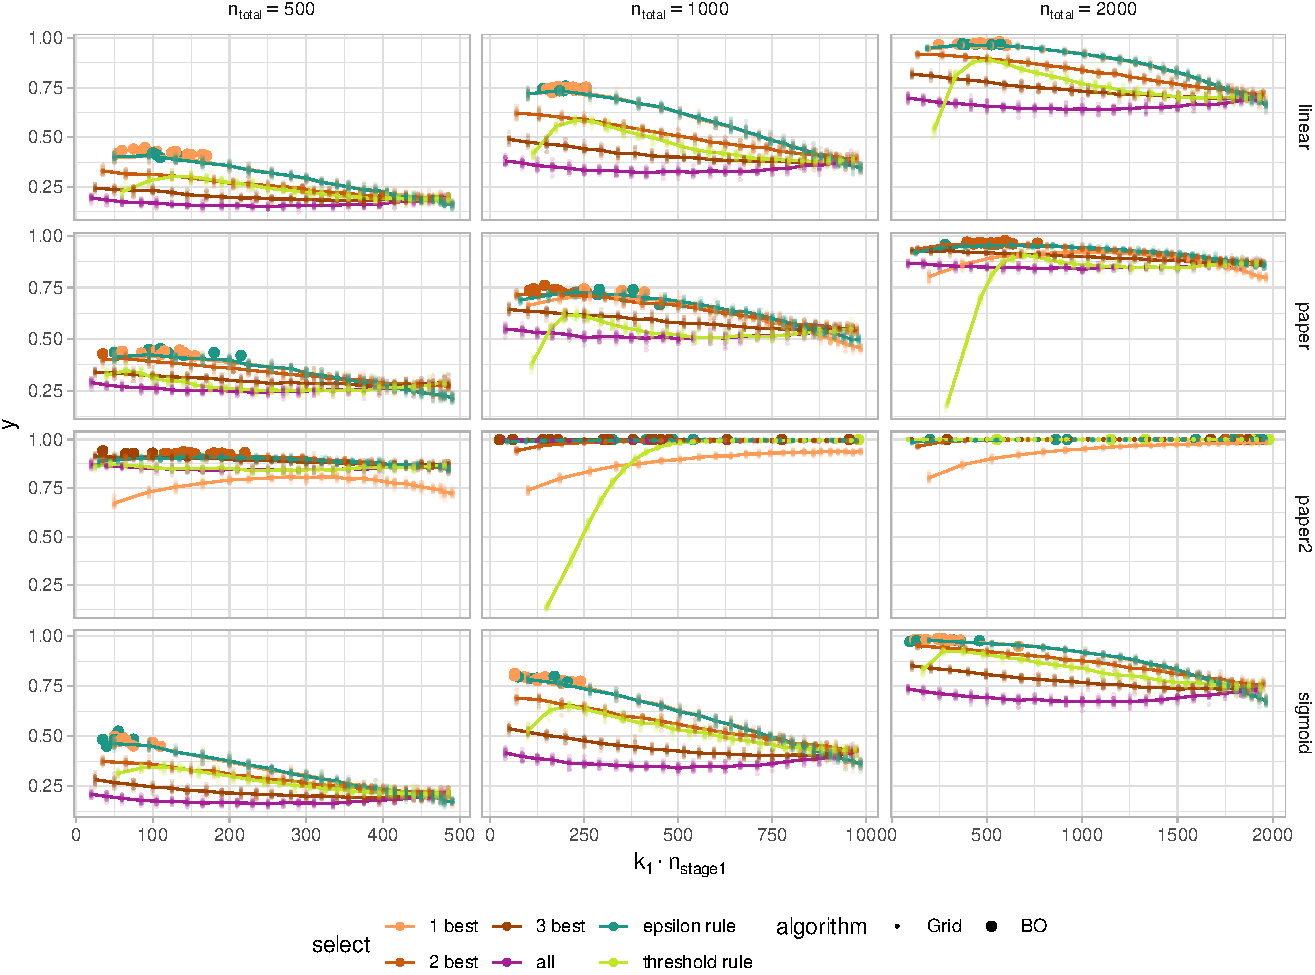
\includegraphics[width=\linewidth]{generated/figures/plot_allbest.pdf}
\caption{Power of the different selection rules. For the epsilon and threshold rule only the curve for the epsilon and threshold value that reached the best power is dispayed.}
\end{center}
\end{figure}


\begin{figure}[htb]
\begin{center}
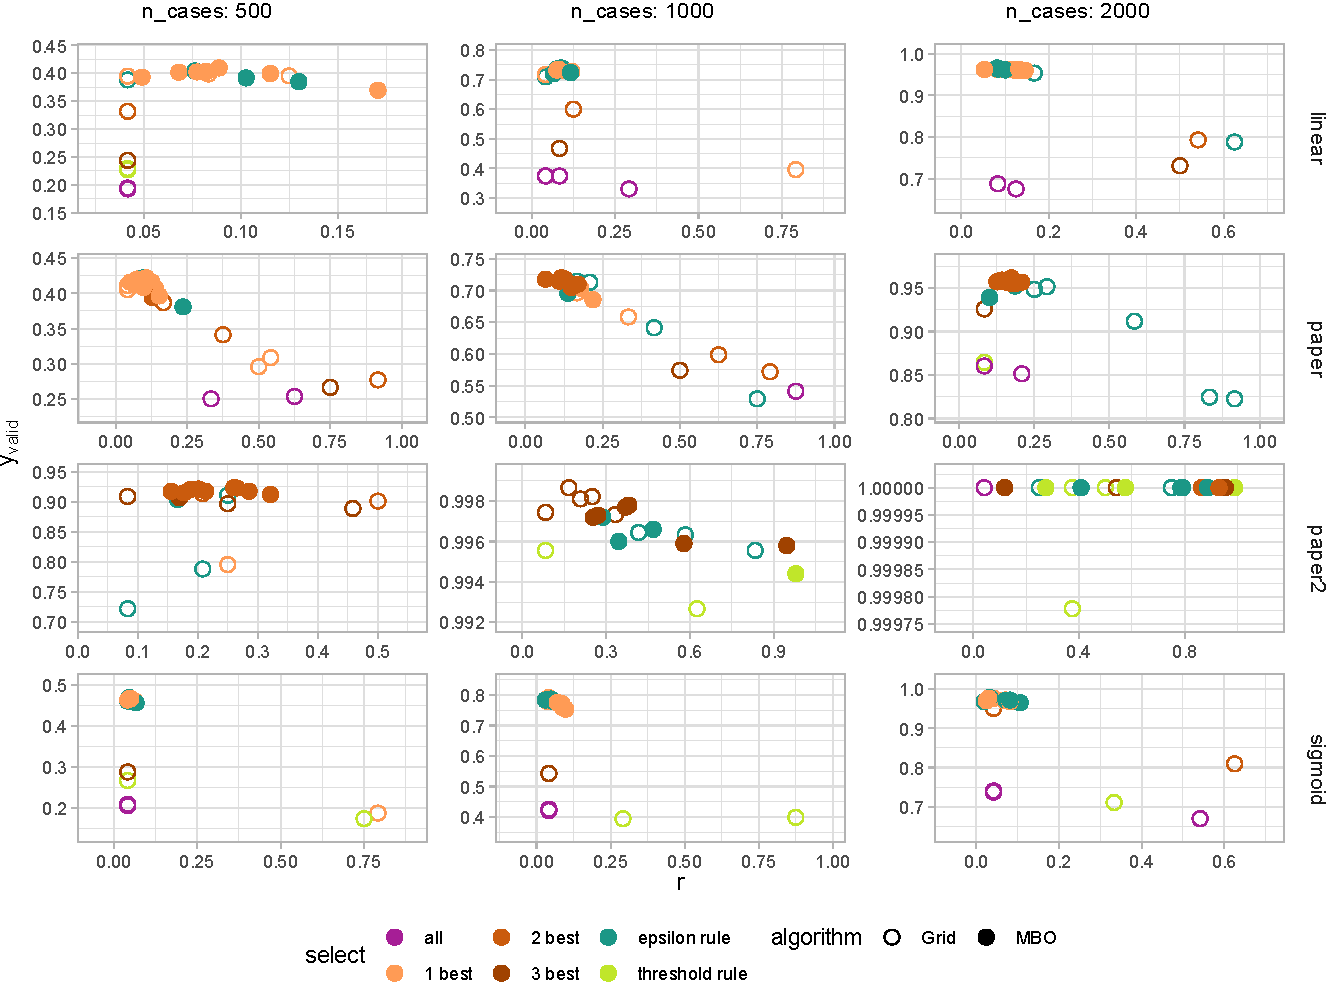
\includegraphics[width=\linewidth]{generated/figures/plot_best_x.pdf}
\caption{Best found $x$-values from MBO runs.}
\end{center}
\end{figure}


\begin{figure}[htb]
\begin{center}
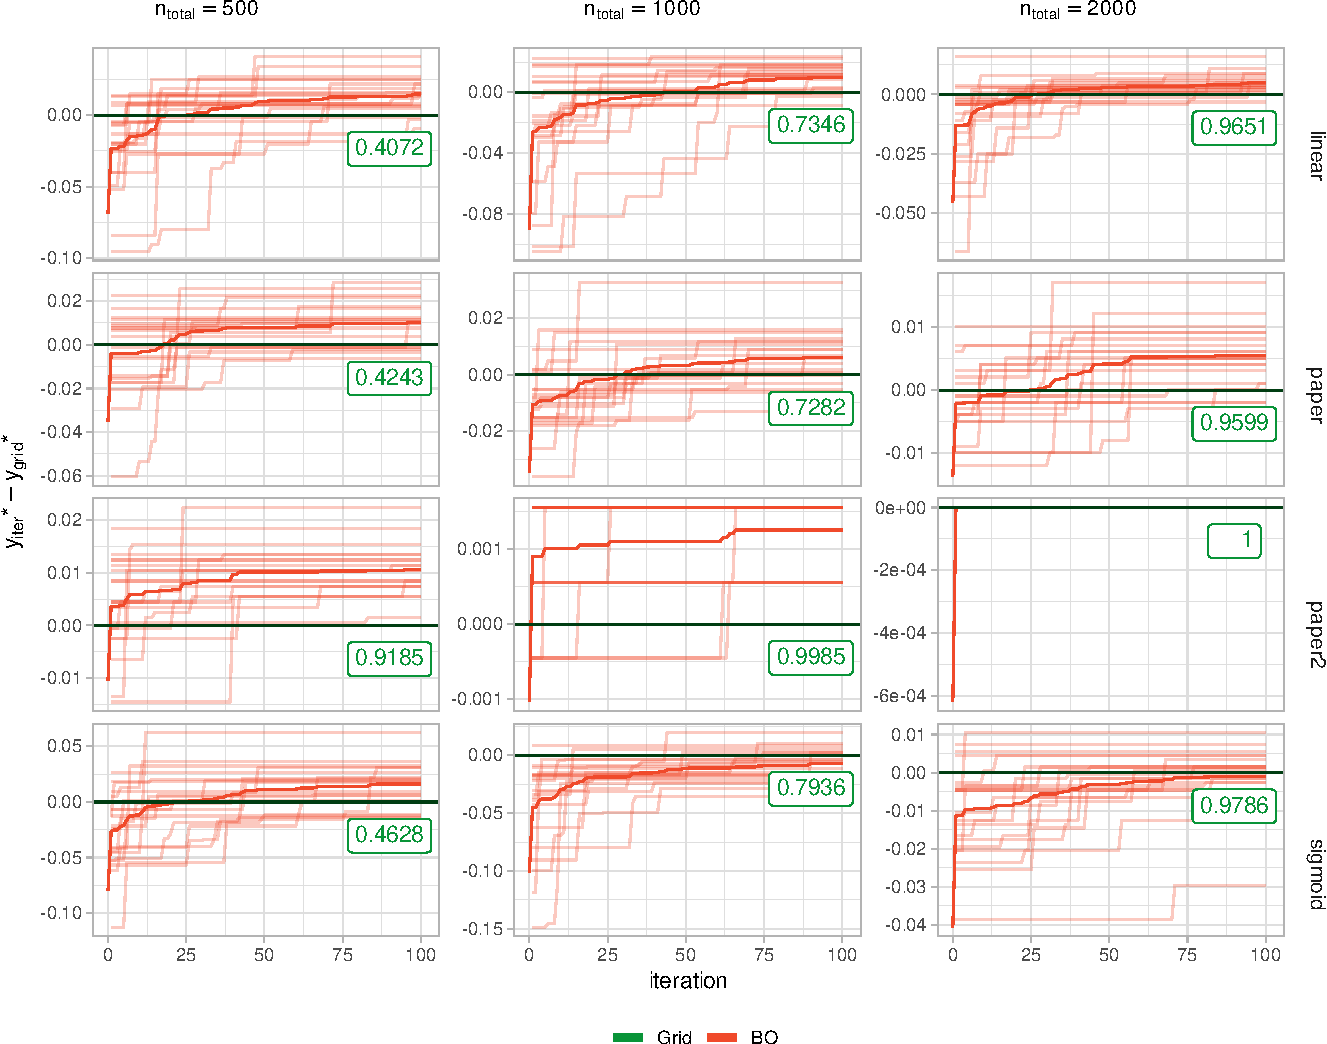
\includegraphics[width=\linewidth]{generated/figures/plot_opt_path.pdf}
\caption{%
  Optimization curves of each optimization run and the mean of all runs drawn as a black line.
  }
\end{center}
\end{figure}

\begin{figure}[htb]
\begin{center}
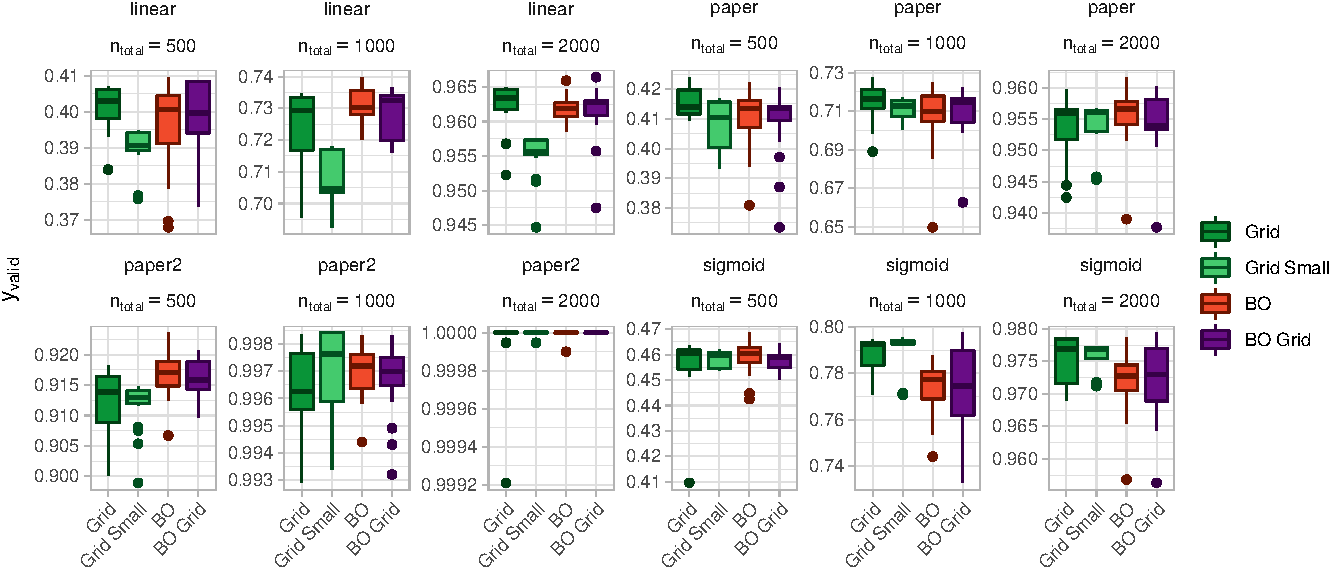
\includegraphics[width=\linewidth]{generated/figures/plot_boxplot_valid_y.pdf}
\caption{%
  Validated performance of both approaches.
  }
\end{center}
\end{figure}

\begin{table}

\caption{Best configurations per ncases and effects}
\centering
\fontsize{6}{8}\selectfont
\begin{tabular}[t]{lrlrrr}
\toprule
effect & n\_cases & select & stage\_ratio & epsilon & mean\_y\\
\midrule
 &  & epsilon rule & 0.042 & 0.000 & 0.401\\

 &  & 1 best & 0.083 &  & 0.405\\

 &  & epsilon rule & 0.083 & 0.000 & 0.407\\

 & \multirow{-4}{*}{\raggedleft\arraybackslash 500} & mbo &  &  & 0.422\\
\cmidrule{2-6}
 &  & epsilon rule & 0.083 & 0.167 & 0.729\\

 &  & 1 best & 0.083 &  & 0.731\\

 &  & epsilon rule & 0.083 & 0.000 & 0.735\\

 & \multirow{-4}{*}{\raggedleft\arraybackslash 1000} & mbo &  &  & 0.744\\
\cmidrule{2-6}
 &  & epsilon rule & 0.083 & 0.000 & 0.965\\

 &  & epsilon rule & 0.083 & 0.333 & 0.965\\

 &  & epsilon rule & 0.083 & 0.167 & 0.965\\

\multirow{-12}{*}{\raggedright\arraybackslash linear} & \multirow{-4}{*}{\raggedleft\arraybackslash 2000} & mbo &  &  & 0.970\\
\cmidrule{1-6}
 &  & 1 best & 0.125 &  & 0.417\\

 &  & epsilon rule & 0.083 & 0.167 & 0.421\\

 &  & epsilon rule & 0.083 & 0.000 & 0.424\\

 & \multirow{-4}{*}{\raggedleft\arraybackslash 500} & mbo &  &  & 0.435\\
\cmidrule{2-6}
 &  & epsilon rule & 0.167 & 0.500 & 0.719\\

 &  & epsilon rule & 0.125 & 0.500 & 0.723\\

 &  & epsilon rule & 0.125 & 0.333 & 0.728\\

 & \multirow{-4}{*}{\raggedleft\arraybackslash 1000} & mbo &  &  & 0.731\\
\cmidrule{2-6}
 &  & 2 best & 0.167 &  & 0.956\\

 &  & 2 best & 0.208 &  & 0.957\\

 &  & 2 best & 0.125 &  & 0.960\\

\multirow{-12}{*}{\raggedright\arraybackslash paper} & \multirow{-4}{*}{\raggedleft\arraybackslash 2000} & mbo &  &  & 0.965\\
\cmidrule{1-6}
 &  & 2 best & 0.208 &  & 0.915\\

 &  & 2 best & 0.292 &  & 0.917\\

 &  & 2 best & 0.250 &  & 0.919\\

 & \multirow{-4}{*}{\raggedleft\arraybackslash 500} & mbo &  &  & 0.929\\
\cmidrule{2-6}
 &  & 3 best & 0.250 &  & 0.998\\

 &  & 3 best & 0.208 &  & 0.998\\

 &  & 3 best & 0.167 &  & 0.998\\

 & \multirow{-4}{*}{\raggedleft\arraybackslash 1000} & mbo &  &  & 1.000\\
\cmidrule{2-6}
 &  & all & 0.042 &  & 1.000\\

 &  & 3 best & 0.042 &  & 1.000\\

 &  & all & 0.083 &  & 1.000\\

\multirow{-12}{*}{\raggedright\arraybackslash paper2} & \multirow{-4}{*}{\raggedleft\arraybackslash 2000} & mbo &  &  & 1.000\\
\cmidrule{1-6}
 &  & epsilon rule & 0.042 & 0.167 & 0.455\\

 &  & 1 best & 0.042 &  & 0.462\\

 &  & epsilon rule & 0.042 & 0.000 & 0.463\\

 & \multirow{-4}{*}{\raggedleft\arraybackslash 500} & mbo &  &  & 0.479\\
\cmidrule{2-6}
 &  & epsilon rule & 0.042 & 0.167 & 0.772\\

 &  & epsilon rule & 0.042 & 0.000 & 0.784\\

 &  & mbo &  &  & 0.787\\

 & \multirow{-4}{*}{\raggedleft\arraybackslash 1000} & 1 best & 0.042 &  & 0.794\\
\cmidrule{2-6}
 &  & epsilon rule & 0.042 & 0.167 & 0.972\\

 &  & 1 best & 0.042 &  & 0.977\\

 &  & mbo &  &  & 0.978\\

\multirow{-12}{*}{\raggedright\arraybackslash sigmoid} & \multirow{-4}{*}{\raggedleft\arraybackslash 2000} & epsilon rule & 0.042 & 0.000 & 0.979\\
\bottomrule
\end{tabular}
\end{table}


\begin{table}

\caption{\label{tab:table_time}Average runtime in hours, for evaluating one grid and one optimization run of MBO.}
\centering
\begin{tabular}[t]{lrrrrrrrrrrrr}
\toprule
\multicolumn{1}{c}{ } & \multicolumn{3}{c}{linear} & \multicolumn{3}{c}{paper} & \multicolumn{3}{c}{paper2} & \multicolumn{3}{c}{sigmoid} \\
\cmidrule(l{3pt}r{3pt}){2-4} \cmidrule(l{3pt}r{3pt}){5-7} \cmidrule(l{3pt}r{3pt}){8-10} \cmidrule(l{3pt}r{3pt}){11-13}
 & 500 & 1000 & 2000 & 500 & 1000 & 2000 & 500 & 1000 & 2000 & 500 & 1000 & 2000\\
\midrule
grid & 55.1 & 60.9 & 60.5 & 62.7 & 63.2 & 204.1 & 59.7 & 64.4 & 67.1 & 54.6 & 52.8 & 61.0\\
mbo & 3.6 & 3.4 & 3.6 & 3.4 & 4.0 & 4.1 & 3.7 & 3.3 & 3.2 & 3.3 & 2.6 & 3.1\\
\bottomrule
\end{tabular}
\end{table}


\subsection{Second level heading}

This is the body text. Please note that cross-references in the body text should be shown as follows:
(Miller, 1900), (Miller and Baker, 1900) or if three or more authors (Miller {\it{et al}}., 1900)
\vspace*{12pt}

\noindent Bullet lists are not allowed. Always use (i), (ii), etc.
\vspace*{12pt}

\noindent Sentences should never start with a symbol.
\vspace*{12pt}

\noindent Names of software packages and website addresses should be written in {\tt{Courier new, i.e. Stata, the R package
MASS, http://www.biometrical-journal.com.}}

\section{Discussion}

% subsection Summary

% subsection Outlook


% \begin{table}[htb]
% \begin{center}
% \caption{The caption of a table.}
% \begin{tabular}{lll}
% \hline
% Description 1 & Description 2 & Description 3\\
% \hline
% Row 1, Col 1 & Row 1, Col 2 & Row 1, Col 3\\
% Row 2, Col 1 & Row 2, Col 2 & Row 2, Col 3\\
% \hline
% \end{tabular}
% \end{center}
% \end{table}
% \begin{equation}
% \left({\theta^{0}_{i}}\atop{\theta^{1}_{i}}\right) \sim N(\theta,\Sigma),\quad {\mathrm{with}}\ 
% {{\theta}} = \left({\theta_{0}}\atop{\theta_{1}}\right)\ {\mathrm{and}}\ \Sigma =
% \left(\begin{array}{cc}
% \sigma^{2}_{0} & \rho\sigma_{0}\sigma_{1}\\
% \rho\sigma_{0}\sigma_{2} & \sigma^{2}_{1}
% \end{array}\right).
% \end{equation}

\noindent This is the body text. Only number equations which are referred to in the text body. If equations
are numbered, these should be numbered continuously throughout the text. Not section wise! Please
carefully follow the rules for mathematical expressions in the ``Instructions to Authors''.

\begin{acknowledgement}
This work was partly supported by Deutsche Forschungsgemeinschaft (DFG) within the Collaborative Research Center SFB 876, A3.
\end{acknowledgement}
\vspace*{1pc}

\noindent {\bf{Conflict of Interest}}

\noindent {\it{The authors have declared no conflict of interest.}} %(or please state any conflicts of interest)

%\section*{Appendix {\it(please insert here, if applicable)}}

%\subsection*{A.1.\enspace Second level heading}

%Please insert appendices before the references.


\bibliographystyle{biometrical}
\bibliography{literature,literature_zotero}

\newpage
\phantom{aaaa}
\end{document}